\section{Pose Representation and Temporal Classifier}
\begin{figure*}[t]
\centering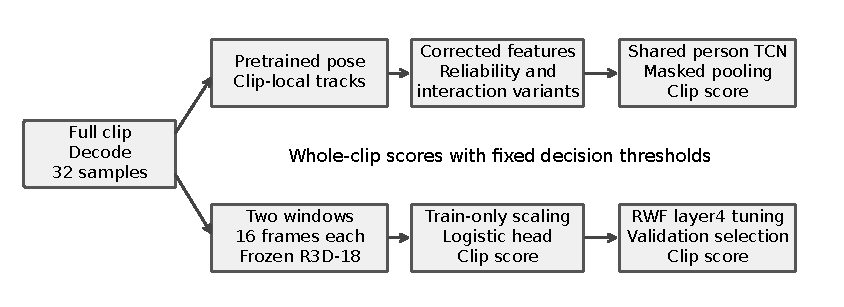
\includegraphics[width=\textwidth]{figures/pipeline.pdf}
\caption{Implemented representation paths. Pretrained estimators supply poses or video embeddings. Pose variants use a shared temporal encoder, while separate crowd and RWF logistic heads use frozen video features. Layer4 fine-tuning is a subsequent RWF development experiment. Each path produces a whole-clip score.}
\label{fig:pipeline}
\end{figure*}
\subsection{Sampling and pose estimation}
For a clip with $N$ decoded frames, we select $T=32$ indices uniformly across the complete sequence. Repeated indices are possible for clips shorter than $T$. Sampling timestamps use the selected indices and recorded frame rate, and velocity denominators have a small positive floor. The pretrained YOLO11n-pose estimator supplies normalized boxes and COCO-17 keypoints \cite{ultralytics}. Extraction uses image size 640, box confidence 0.2, joint-validity threshold 0.25, and at most 100 detections per sampled image. Estimator weights and settings are fixed for each recorded extraction signature.

Let $\mathbf{q}_{tpj}\in\R^2$ be the image-normalized coordinates of joint $j$ for track $p$ at sampled time $t$, and let $c_{tpj}$ be its confidence. Let $m_{tp}\in\{0,1\}$ denote an observed track. Joint validity is
\begin{equation}
v_{tpj}=m_{tp}\,\mathbf{1}[c_{tpj}\geq 0.25].
\label{eq:valid}
\end{equation}
Detector confidence expresses estimator output and is not a calibrated probability of joint correctness or violence. Missing detections do not establish absence of violent activity.

\subsection{Clip-local association and track packing}
Hungarian assignment \cite{kuhn1955} associates boxes within each clip using a cost combining intersection-over-union (IoU) and normalized center distance. A candidate link is permitted when IoU is at least 0.1 or center distance is at most 0.18. Its cost is $(1-\mathrm{IoU})+2d$, where $d$ is center distance. Tracks remain eligible through two missing sampled observations, and unmatched detections receive new identifiers. IDs reset at the beginning of each clip.

The pipeline retains $P=8$ tracks with the largest sum of observed keypoint-confidence signal. Empty slots contain zero values and an absent mask. The packed raw tensors have dimensions $T\times P\times17\times3$ for keypoints and $T\times P\times4$ for boxes. Association can fragment under occlusion, rapid movement, or a camera cut, and the eight-track limit can discard people. This implementation has no independently measured identity-switch rate or person-attribution accuracy.

\subsection{Continuous body origin}
Body normalization requires an origin. With both hip joints valid, the observed midpoint $\mathbf{h}_{tp}$ supplies that origin. Let $\mathbf{b}_{tp}$ be the box center. The legacy implementation switches directly to $\mathbf{b}_{tp}$ when a hip is missing. A change in the difference between hip and box centers can then appear as joint motion even if body motion is unchanged.

The corrected implementation estimates a continuous hip-to-box offset inside each uninterrupted observed track segment. At reliable hip anchors, the offset is $\mathbf{o}_{tp}=\mathbf{h}_{tp}-\mathbf{b}_{tp}$. Linear interpolation in sampled time fills offsets at missing-hip observations, with nearest-anchor extension at segment boundaries. For segments without reliable hip anchors, box center remains the fallback. The origin is
\begin{equation}
\mathbf{a}_{tp}=
\begin{cases}
\mathbf{h}_{tp}, & \text{both hips valid},\\
\mathbf{b}_{tp}+\widetilde{\mathbf{o}}_{tp}, & \text{anchors exist},\\
\mathbf{b}_{tp}, & \text{no hip anchor in segment}.
\end{cases}
\label{eq:center}
\end{equation}
Interpolation does not fill absent person observations. It uses the complete observed segment and is therefore an offline operation. Future anchors can influence an earlier missing-hip origin. The procedure uses no class labels, but it remains sensitive to box jitter, bad hip estimates, and association errors. The matched centering experiment fits all classifiers afresh for both schemas.

\subsection{Body coordinates and velocity}
Let $s_{tp}$ be the normalized box-diagonal length, floored at 0.03. We calculate body-centered coordinates
\begin{equation}
\mathbf{x}_{tpj}=v_{tpj}\,\operatorname{clip}
\left((\mathbf{q}_{tpj}-\mathbf{a}_{tp})/s_{tp},-3,3\right).
\end{equation}
Joint velocity uses actual sampled-time differences and only jointly valid neighboring observations:
\begin{equation}
\mathbf{u}_{tpj}=v_{tpj}v_{t-1,p,j}\,
\operatorname{clip}\left(
\frac{\mathbf{x}_{tpj}-\mathbf{x}_{t-1,p,j}}{\Delta t_t},-10,10\right),
\label{eq:velocity}
\end{equation}
where $\Delta t_t$ is floored at $10^{-3}$ s and the first velocity is zero. The baseline concatenates two coordinates and two velocity components for each of 17 joints, giving 68 channels per person and time.

The reliability variant multiplies positions and velocities by current joint confidence and appends 17 masked confidence channels and 17 validity channels. This yields 102 channels. The confidence weighting is a fixed feature operation rather than a learned uncertainty model. Validity information remains predictive even when a joint coordinate itself is unavailable.

\subsection{Nearest-person interaction features}
Interactions use shared image-normalized origins before individual scale normalization. For each observed person, the nearest other observed origin is selected by Euclidean distance. Let its offset be $\mathbf{r}_{tp}$ and its relative origin velocity be $\dot{\mathbf{r}}_{tp}$. The eight interaction channels are distance, two offset components, two relative-velocity components, signed radial relative velocity, normalized neighbor count, and neighbor presence. Radial relative velocity is
\begin{equation}
\gamma_{tp}=\operatorname{clip}
\left(\frac{\mathbf{r}_{tp}^{\mathsf T}\dot{\mathbf{r}}_{tp}}
{\max(\|\mathbf{r}_{tp}\|,10^{-4})},-10,10\right).
\end{equation}
Each origin velocity is the sampled-time difference of that person's image-normalized origin, clipped componentwise to $[-10,10]$ and set to zero unless that person is observed at both adjacent samples. The relative velocity subtracts the current person's origin velocity from the selected neighbor's origin velocity. It is not obtained by differentiating the nearest-neighbor offset across possible neighbor changes. Negative radial velocity indicates approach under this offset convention. Neighbor count divides the number of other observed people by $P-1$. The interaction-only variant has 76 channels, and the combined reliability/interaction variant has 110. When no neighbor is observed, the interaction vector is zero.

These descriptors use two-dimensional apparent geometry. Perspective means that image distance is not physical separation, and the nearest visible origin need not be the person participating in an interaction. Camera motion affects origin velocity. We therefore describe these as candidate interaction cues and do not interpret them as reliable contact, intent, or aggressor measurements.

\begin{table}[t]
\caption{Pose feature variants. Parameter counts use the shared 48-channel temporal encoder and coverage-enabled classifier.}
\label{tab:variants}\centering
\begin{tabular}{lrr}
\toprule Variant & Input channels & Parameters\\
\midrule Baseline & 68 & 36,001\\
Reliability & 102 & 37,633\\
Interactions & 76 & 36,385\\
Combined & 110 & 38,017\\
\bottomrule
\end{tabular}
\end{table}

\subsection{Temporal encoding and person pooling}
The classifier shares one temporal encoder across person slots. A $1\times1$ convolution projects each person's feature sequence to 48 hidden channels. Three residual blocks use temporal kernel width 3 and dilations 1, 2, and 4. Each block contains a dilated convolution, Gaussian error linear unit, dropout of 0.2, a pointwise convolution, and a second activation. Symmetric padding preserves the time dimension. The observation mask applies after input projection and after each residual block.

For encoded values $\mathbf{z}_{tp}\in\R^{48}$, each person descriptor averages only observed times:
\begin{equation}
\overline{\mathbf{z}}_p=
\frac{\sum_t m_{tp}\mathbf{z}_{tp}}
{\max(1,\sum_t m_{tp})}.
\end{equation}
Mean and componentwise maximum across observed people form a 96-dimensional set descriptor. Concatenating observed-track coverage, $\rho=(TP)^{-1}\sum_{t,p}m_{tp}$, gives 97 classifier inputs. A 48-unit hidden layer with activation and dropout feeds one binary logit. The sigmoid produces a clip score, and a validation-selected threshold produces the decision.

Pooling is invariant to person-slot ordering, but it can discard which specific person or interaction generated the signal. Coverage is a direct detection cue. Masks, standardized missing-joint values, confidence, neighbor availability, and track packing provide indirect cues as well. Consequently, even the baseline is not a motion-only representation isolated from estimator behavior. Table~\ref{tab:variants} also shows that changed input dimensions change nominal parameter count, although all variants share the encoder family and training budget.
